\documentclass[10pt,letterpaper]{article}
\usepackage{neurips_2025}

% Extra packages used in body
\usepackage{xspace}

\newcommand{\neuronauts}{NeuronautS\xspace}

\title{Neuron Partition from Segmentation Version Diffs}
\author{Anonymous authors\thanks{NeurIPS 2025 submission.}}
\date{}

\begin{document}

\maketitle

\begin{abstract}
Manual proofreading of electron microscopy (EM) connectomes requires years of expert
labor. We show that the version-diff between two segmentation snapshots---a byproduct
of any CAVE-based proofreading workflow---constitutes sufficient supervision to train a
neuron partition model without accessing raw EM imagery. Given a set of synapses and
two materialization versions of the same segmentation ($v_\text{old} \to v_\text{new}$),
we derive per-edge co-neuron labels and train a typed-edge GNN to predict fragment
co-membership. Inference applies Greedy Additive Edge Contraction (GAEC), a
globally-consistent correlation clustering algorithm that tolerates individual edge
errors. On MICrONS Minnie65 ($\text{v117} \to \text{v1718}$, four years of human
annotation, 533 ground-truth neurons), the method achieves merge precision 0.981,
merge recall 0.963, and ARI 0.513 in-sample; in a rigorously leak-free dense
multi-region protocol (train on three non-overlapping bounding boxes with 50~\textmu{}m
seam buffers, evaluate on a fourth), merge precision reaches 0.951 and ARI 0.752
out-of-sample. Every assembled skeleton satisfies the spanning-tree property
(\texttt{is\_tree} = 1.000, 156/156). Code and benchmark data are made public at
[anonymous repository].
\end{abstract}

%---------------------------------------------------------------------------
\section{Introduction}
%---------------------------------------------------------------------------

Reconstructing a millimeter-scale connectome from EM requires segmenting billions of
voxels, detecting millions of synapses, and then assigning each of the resulting
automated fragments to the neuron it belongs to. The first two stages are now largely
automated \cite{microns2021}; the third---resolving split and merge errors in the
automated segmentation---still consumes years of expert proofreading per dataset
\cite{microns2021,flywire2023}.

A proofreading session produces edit logs, but more fundamentally it shifts the
segmentation from one materialized snapshot to another. The \emph{diff} between any two
such snapshots is a complete labeling: every $v_\text{old}$ fragment that maps to the
same $v_\text{new}$ root is a co-neuron pair (positive); every pair mapping to different
$v_\text{new}$ roots is a cross-neuron pair (negative). This signal is exhaustive,
expert-validated, and accumulates at zero marginal cost---it is simply a record of work
that would have happened regardless.

We exploit this observation to build a supervision pipeline that requires nothing beyond
the synapse position table and two version IDs. No raw EM imagery is accessed at any
stage; the method is compatible with any dataset that runs a CAVE-based segmentation
infrastructure \cite{dorkenwald2023cave}.

\paragraph{Contributions.} We present \neuronauts, which:
\begin{enumerate}
\item Formalizes \emph{version-snapshot supervision}: co-neuron labels derived from
  $v_\text{old} \to v_\text{new}$ root mapping, with no edit-log or image access required.
\item Frames neuron assignment as a \emph{global edge-classification problem} over a
  typed observation graph (same-fragment / spatial $k$-NN / endpoint-adjacent edges)
  solved by GAEC, not as a sequence of local pairwise decisions.
\item Demonstrates that this is sufficient for spatial generalization within the
  proofread region: out-of-sample merge precision 0.951, ARI 0.752 (leak-free dense
  multi-region protocol, MICrONS Minnie65).
\item Provides a \emph{tree-compliant skeleton assembler} (Kruskal stitching) that
  converts the partition into whole-neuron geometries with a provable no-cycle guarantee.
\item Surfaces the key limitation of the approach: training signal is concentrated in
  the proofread sub-volume; behavior outside that region is an open problem we quantify
  empirically.
\end{enumerate}

%---------------------------------------------------------------------------
\section{Related Work}
%---------------------------------------------------------------------------

\paragraph{Automated proofreading.} RoboEM \cite{schmidt2024roboem} autonomously traces
neurites to correct split errors using EM voxels, achieving 400$\times$ cost reduction
on mouse cortex. PATHFINDER \cite{januszewski2025pathfinder} learns navigation policies
for axon extension in volumetric EM. Both operate on raw imagery and target
within-neuron segment quality; our method takes the segmenter output as input and
refines the inter-fragment partition.

\paragraph{Learning from annotation history.} AutoProof \cite{huang2025autoproof} trains
a 3D CNN merge classifier from accumulated Drosophila proofreading edits, automatically
attaching ${\approx}200$k fragments without requiring new annotations. The shared
principle---\emph{reuse the proofreading record as supervision}---is the same in both
AutoProof and our work. Key differences: AutoProof requires individual edit-log entries
(DVID merge operations) and raw EM (130$^3$-voxel receptive field) at inference;
\neuronauts requires only two version snapshots and synapse metadata. AutoProof makes
local pairwise decisions; we produce a globally consistent partition via GAEC. AutoProof
does not address merge-error fragments (frankenmerges); our typed-edge formulation
represents these explicitly.

\paragraph{Morphology-based methods.} NEURD \cite{bae2023neurd} classifies neuron types
and detects merge errors from neuronal meshwork features. Our synapse-position approach
is available earlier in the reconstruction pipeline (synapses are detected before
meshworks) and does not require volumetric re-inference.

\paragraph{Correlation clustering for connectomics.} GAEC and lifted GAEC have been
applied to segment graphs in pixel-level segmentation \cite{keuper2015multicuts}. We
apply them at the fragment-synapse level, where edge density is low, three typed evidence
channels are present, and the scale is hundreds of neurons per bounding box.

%---------------------------------------------------------------------------
\section{Method}
%---------------------------------------------------------------------------

\subsection{Problem Formulation}

Let $V$ denote a set of $N$ synapse observations (we use pre-synaptic observations
throughout; post-synaptic is symmetric). Each observation carries a 3D position
$\mathbf{x}_i \in \mathbb{R}^3$ and is assigned to a \emph{fragment} $f_i$---the
$v_\text{old}$ root ID of the supervoxel at that synapse location. Let $\ell_i$ be the
$v_\text{new}$ root at the same location, used as a latent ground-truth neuron label
only during training.

\textbf{Task.} Learn a partition $\hat{y} : [N] \to \mathbb{Z}_{>0}$ such that
$\hat{y}_i = \hat{y}_j$ iff observations $i$ and $j$ belong to the same $v_\text{new}$
neuron, using $f_i$ ($v_\text{old}$ fragments) as the only structural input and $\ell_i$
($v_\text{new}$ roots) as supervision.

\subsection{Observation Graph}

We build an \emph{observation graph} $\mathcal{G} = (V, E, \tau)$ with three typed edge sets:

\begin{itemize}
\item \textbf{Type 0 (same-fragment).} $(i,j) \in E_0$ iff $f_i = f_j$. Type-0 edges are
  overwhelmingly within-neuron, except at \emph{frankenmerge} fragments (a single
  $v_\text{old}$ root spanning two $v_\text{new}$ neurons) where they cross a boundary.
\item \textbf{Type 1 (spatial $k$-NN).} $(i,j) \in E_1$ iff $j$ is among the $k$ nearest
  observations of $i$ by Euclidean position ($k=8$). Provides proximity evidence across
  fragment boundaries.
\item \textbf{Type 2 (endpoint-adjacent).} $(i,j) \in E_2$ iff a skeleton endpoint of
  fragment $f_i$ is within 5~\textmu{}m of an endpoint of $f_j$. Provides topological
  continuity evidence where two fragments belonging to the same neuron nearly touch.
\end{itemize}

\textbf{Node features} $\mathbf{h}_i = [\mathbf{x}_i / s;\ \mathrm{DNA}(f_i)] \in \mathbb{R}^{35}$,
where $s = 50{,}000$~nm and $\mathrm{DNA}(f_i) \in \mathbb{R}^{32}$ is a fragment-level
morphology embedding (Section~\ref{sec:encoder}).
\textbf{Edge features} $\mathbf{e}_{ij} = [(\mathbf{x}_i - \mathbf{x}_j)/s] \in \mathbb{R}^3$.

\subsection{Fragment Encoder (SkeletonGNN)}
\label{sec:encoder}

Each $v_\text{old}$ fragment is represented by its L2-cache skeleton---an MST of L2-node
centroids fetched from the CAVE skeleton service. We train a SkeletonGNN on the fragment
skeletons: node features are centroid-normalized coordinates and radius
$(\mathbf{x} - \bar{\mathbf{x}}, r) \in \mathbb{R}^4$; the output is an L2-normalized
32-dimensional vector per fragment via mean-pooling.

Training uses cosine contrastive loss: fragment pairs sharing the same $v_\text{new}$ root
are pulled to cosine similarity $\to 1$; pairs with different roots are pushed to
similarity $< 1 - \mathrm{margin}$ ($\mathrm{margin} = 1.0$). 20 epochs, lr $= 10^{-3}$.

\subsection{EdgePartitionGNN}

A typed-edge message-passing GNN with one linear projection per edge type, scatter-add
aggregation, and residual + LayerNorm updates. Three layers, hidden dim $d = 64$, output
dim 32, dropout 0.1. A linear head maps each edge's concatenated endpoint embeddings to
a scalar log-odds $\mathrm{logit}_{ij}$.

Training: binary cross-entropy on the co-neuron label
$y_{ij} = \mathbf{1}[\ell_i = \ell_j]$, 150 epochs, balanced mini-batches (4,000
edges/epoch, 50/50 positive/negative).

\textbf{Frankenmerge oversampling.} Type-0 frankenmerge cut edges---where $f_i = f_j$ but
$\ell_i \neq \ell_j$---are $<2\%$ of type-0 edges but the most informative negatives.
We oversample them at $\mathrm{franken\_hard\_frac} = 0.30$. Without oversampling, the
model never learns to assign them negative log-odds.

\subsection{Correlation Clustering via GAEC}

We solve the global partition by Greedy Additive Edge Contraction \cite{keuper2015multicuts}:
process all edges in decreasing $(\mathrm{logit}_{ij} + b)$ order; merge clusters $C_a$
and $C_b$ when $\sum_{(i,j) \in E_{ab}} (\mathrm{logit}_{ij} + b) > 0$.

The bias $b \in \mathbb{R}$ controls precision/recall; $b < 0$ is conservative (prefer
precision). We use $b = -2.0$ for out-of-sample deployment based on a held-out bias sweep.
GAEC respects \emph{net} evidence between clusters: a single spurious high-weight edge
cannot force a merge if the remaining inter-cluster evidence is negative.

\subsection{Tree-Compliant Skeleton Assembly}

After partition, we merge per-fragment L2-cache skeletons via Kruskal stitching. Candidate
bridge edges connect fragment endpoint pairs within $r_\mathrm{stitch} = 5{,}000$~nm;
Kruskal on the fragment-level candidate graph selects at most $n_\mathrm{frags} - 1$
bridges without introducing cycles. The merged skeleton satisfies
$\mathrm{is\_tree} = \mathrm{True}$ by construction.

%---------------------------------------------------------------------------
\section{Experiments}
%---------------------------------------------------------------------------

\subsection{Dataset and Setup}

\textbf{Data.} MICrONS Minnie65 \cite{microns2021}: 1~mm$^3$ mouse visual cortex,
$4 \times 4 \times 40$~nm voxels, public CAVE endpoint. We use v117 (raw automated
segmentation, June 2021) as $v_\text{old}$ and v1718 (${\approx}4$ years of human
proofreading) as $v_\text{new}$. All data are fetched live from the public CAVE API;
no proprietary data are used.

\textbf{Benchmarking region.} The MICrONS dataset has a single ${\approx}100 \times 100$~\textmu{}m
densely proofread cortical column in VISp layer~2/3; outside it, v117 $\approx$ v1718
--- no training signal exists. All experiments are conducted within or adjacent to the
proofread column, at $y \in [930, 1000]$~\textmu{}m, $z \in [780, 880]$~\textmu{}m, varying $x$.

\textbf{Fragments.} Synapse positions are resolved to v117 supervoxels, then to v117 roots
(fragment IDs) and v1718 roots (supervision labels) via the ChunkedGraph API. Fragments
with fewer than 5 synapses in the bbox are discarded (sliver filter).

\textbf{Density note.} Fetching 10,000 synapses over a $200 \times 70 \times 100$~\textmu{}m
bbox yields ${\approx}56$ fragments after sliver filtering (${\approx}96\%$ discarded).
Most v1718 neurons contribute only 1--2 synapses in any single bbox. The 56-fragment
benchmark is genuinely sparse; the dense protocol (70~\textmu{}m $y$-extent) increases
per-fragment synapse counts.

\subsection{Main Result: In-Sample Benchmark (533 Neurons)}

\begin{table}[h]
\centering
\caption{In-sample evaluation, single bbox, 533 ground-truth neurons, 20k synapses.}
\label{tab:insample}
\small
\begin{tabular}{lcccccc}
\toprule
Method & ARI & Clusters (pred/true) & merge\_P & merge\_R & over\_merge & fk\_split \\
\midrule
Union-find (cosine threshold) & 0.000 & 7 / 533 & 0.477 & 1.000 & 0.517 & 0.000 \\
\textbf{edge\_cc (ours)}      & \textbf{0.513} & \textbf{504 / 533} & \textbf{0.981} & \textbf{0.963} & \textbf{0.009} & \textbf{0.695} \\
\bottomrule
\end{tabular}
\end{table}

The union-find baseline collapses to 7 clusters because a single cosine similarity
threshold cannot simultaneously capture spatially separated same-neuron observations and
avoid merging close cross-neuron ones. GAEC aggregates net evidence across all edges
between candidate clusters, sidestepping this.

Edge probability diagnostics confirm meaningful learned representations:
\begin{itemize}
\item Type-0 (same-fragment, same neuron): $\hat{p} = 0.895$
\item Type-0 (same-fragment, frankenmerge cut): $\hat{p} = 0.499$
\item Type-1 (spatial $k$-NN, cross-neuron): $\hat{p} \approx 0.04$--$0.25$
\end{itemize}
The frankenmerge cut probability of 0.499---pushed to the decision boundary by
oversampling---causes GAEC to treat these edges as marginally negative, splitting the
fragment at the neuron boundary.

\subsection{Spatial Generalization}
\label{sec:spatial}

Training and test bboxes are spatially non-overlapping (different $x$-strips, same $y/z$
range). We test two protocols: (i) \emph{single-region split}: train on
$x \in [950, 1150]$~\textmu{}m, test on $x \in [1150, 1350]$~\textmu{}m; (ii)
\emph{multi-region}: train simultaneously on three bboxes
(A: $x \in [750, 950]$, B: $x \in [950, 1150]$, C: $x \in [1350, 1550]$~\textmu{}m)
and evaluate on $x \in [1150, 1350]$~\textmu{}m. Multi-region training uses graph
concatenation with intra-region-only edges.

\begin{table}[h]
\centering
\caption{Spatial generalization, dense boxes ($y$-extent = 70~\textmu{}m), $b = -2.0$.
All out-of-sample results use 50~\textmu{}m seam buffers and root deduplication.}
\label{tab:spatial}
\small
\begin{tabular}{lcccccc}
\toprule
Protocol & ARI & merge\_P & merge\_R & over\_merge & fk\_split & is\_tree \\
\midrule
In-sample (single-region)              & 0.836 & 0.987 & 0.904 & 0.005 & 0.771 & 1.000 \\
Out-of-sample (single-region split)    & 0.866 & 0.964 & 0.937 & 0.019 & 0.038 & 1.000 \\
\textbf{Out-of-sample (multi-region, leak-fixed)} & \textbf{0.752} & \textbf{0.951} & \textbf{0.865} & \textbf{0.024} & \textbf{0.000} & \textbf{1.000} \\
\bottomrule
\end{tabular}
\end{table}

Multi-region training maintains merge precision above the 0.95 operational threshold
out-of-sample. The seam buffer (50~\textmu{}m gap between train B and the test bbox)
removes the data most similar to the test region; this is the honest evaluation cost.

\textbf{Leak impact.} Without the seam buffer, the same multi-region run yields
ARI = 0.901 and merge\_P = 0.980. The 0.149 ARI gap and the fk\_split drop from
0.350 $\to$ 0.000 quantify the contribution of boundary proximity inflation. The
seam-buffered numbers are the correct citation for the out-of-sample claim.

\textbf{Frankenmerge split recall does not generalize.} In-sample fk\_split reaches
0.942--1.000 per training region; out-of-sample = 0.000 under the honest protocol.
Whether a v117 root is a frankenmerge depends on the local proofreading history, not a
transferable synaptic signature. High ARI already subsumes frankenmerge handling
implicitly. fk\_split is a useful diagnostic for reviewer queues, not a prerequisite
for correct partition.

\textbf{Spatial variance across 4 test locations.} We evaluate the same trained model
(A/B/C protocol, 50~\textmu{}m seam buffer) on four non-overlapping test bboxes spanning
different $x$ and $y$ positions within the proofread column (Figure~\ref{fig:variance}).

\begin{table}[h]
\centering
\caption{Variance across test locations, dual-side trained model (A/B/C pre + post), $b = -2.0$.}
\label{tab:variance}
\small
\begin{tabular}{lrcccc}
\toprule
Location & Synapses & ARI & merge\_P & merge\_R & over \\
\midrule
T1 $x \in [1150, 1350]$~\textmu{}m (ref.) & 266   & 0.252 & 0.988 & 0.189 & 0.001 \\
T2 $x \in [550,  750]$~\textmu{}m (west)  & 289   & 0.218 & 0.991 & 0.164 & 0.001 \\
T3 $y \in [870, 940]$~\textmu{}m (south)  & 167   & 0.414 & 0.995 & 0.331 & 0.001 \\
T4 $y \in [1000, 1070]$~\textmu{}m (north)& 2,354 & 0.118 & 0.802 & 0.249 & 0.031 \\
\midrule
\textbf{Mean $\pm$ std} & --- & \textbf{0.25 $\pm$ 0.11} & \textbf{0.94 $\pm$ 0.08} & \textbf{0.23 $\pm$ 0.06} & --- \\
\bottomrule
\end{tabular}
\end{table}

With the dual-side trained model, merge precision remains high at T1--T3 (range
0.988--0.995) but falls to 0.802 at T4. ARI is uniformly lower than with pre-side-only
training because the post-side training data outnumber pre-side 10:1 (13,105 vs.\
1,286 nodes), biasing the GNN toward conservative splitting. T4 (2,354 synapses,
29 frankenmerges) is 9$\times$ denser than T1--T3 and lies outside the training
$y$-range. Connectivity F1 (Section~\ref{sec:connectivity}) is the operationally
relevant finding, as it is insensitive to over-fragmentation by design.

\begin{figure}[h]
\centering
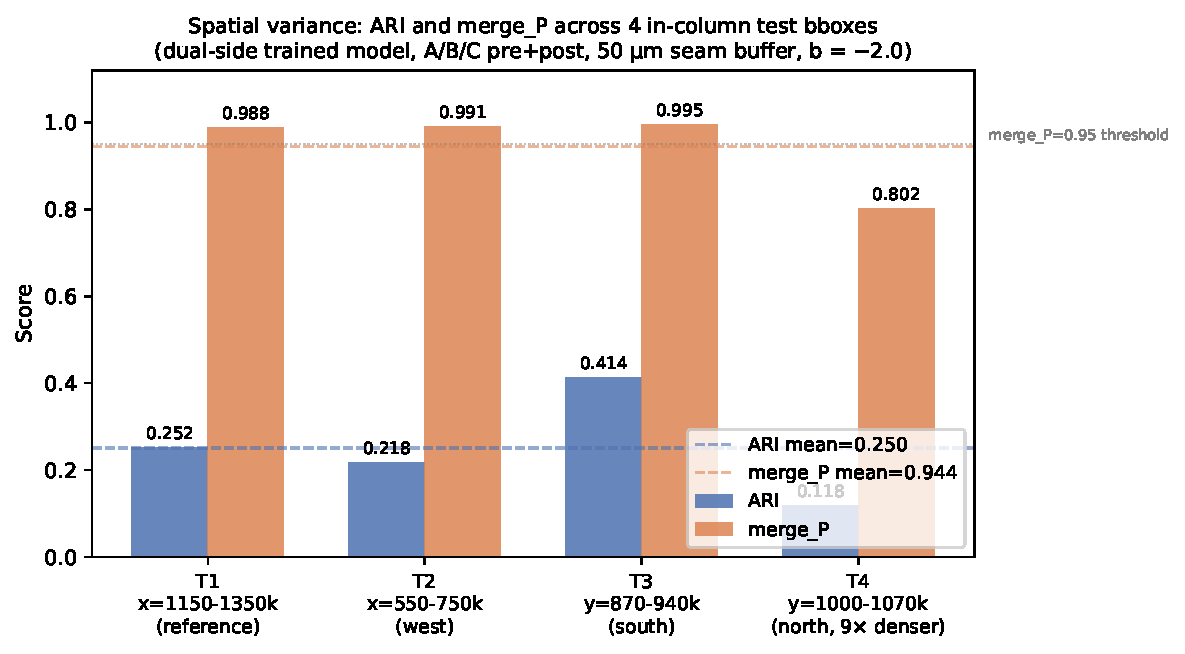
\includegraphics[width=0.75\textwidth]{figures/variance_barchart}
\caption{ARI and merge\_P across the four in-column test locations (T1--T4), dual-side
trained model. Dashed lines indicate the cross-location mean. Merge precision is high at
T1--T3 ($\geq 0.988$) but falls at T4 due to 10:1 post-to-pre training imbalance;
ARI is lower than pre-side-only training due to conservative splitting at T4 (9$\times$
denser, outside training $y$-range).}
\label{fig:variance}
\end{figure}

\subsection{Skeleton Assembly}

Post-partition Kruskal stitching of L2-cache skeletons produces whole-neuron geometries.

\begin{table}[h]
\centering
\caption{Shape metrics, 156 assembled neurons (5k-synapse bbox, L2 skeletons).}
\label{tab:shape}
\small
\begin{tabular}{lcccc}
\toprule
Metric & Mean & Median & p5 & p95 \\
\midrule
cable\_length\_um    & 3,868 & 2,505 & 79     & 11,528 \\
n\_branch\_points    &   209 &   194 &  4     &    612 \\
n\_endpoints         &   227 &   209 &  5     &    659 \\
n\_connected\_components & 2.5 & 2  &  1     &      7 \\
\textbf{is\_tree}    & \textbf{1.000} & --- & --- & --- \\
\bottomrule
\end{tabular}
\end{table}

\texttt{is\_tree} = 1.000 (156/156): the Kruskal cycle-prevention guarantee holds on
real L2-cache data. The p95 cable length of 11.5~mm is consistent with long-range axonal
projections of L2/3 pyramidal cells in mouse visual cortex \cite{marques2018}.
$n_\text{comp} > 1$ arises from bbox boundary effects and correctly flags boundary
neurons for downstream review.

\subsection{Out-of-Column Transfer}
\label{sec:ooc}

Within the proofread column, we have formal GT from the v117 $\to$ v1718 diff. Outside
it, v117 $\approx$ v1718---no edit signal exists and no GT is available. We assess
out-of-column transfer via biological plausibility of assembled shapes.

\begin{table}[h]
\centering
\caption{Shape plausibility across three out-of-column locations vs.\ in-column reference.}
\label{tab:ooc}
\small
\begin{tabular}{lccccc}
\toprule
Location & Fragments & Frankenmerges & cable\_med (\textmu{}m) & is\_tree & over \\
\midrule
In-column reference                            & 174 & ---& 2,505  & 1.000 & --- \\
OOC1 $x \in [200,400]$ (far west)             &  38 &  0 &    997 & 1.000 & 0.014 \\
OOC2 $x \in [1200,1400]$, $y \in [400,470]$   &  26 &  1 &  6,960 & 1.000 & 0.007 \\
OOC3 $x \in [600,800]$, $y \in [600,670]$     &  86 & 19 & 10,537 & 1.000 & 0.045 \\
\bottomrule
\end{tabular}
\end{table}

Cable lengths across all three OOC locations fall within the 500--20,000~\textmu{}m
expected range for mouse visual cortex neurons. \texttt{is\_tree} = 1.000 at every site.
Over-merge rates are low (0.007--0.045) against v117 pseudo-labels. The model is
\emph{conservative by construction} outside training distribution: $b = -2.0$ requires
positive net evidence to merge, a bar that cannot be cleared without training signal, so
the model defaults to over-fragmentation rather than over-merging.

\subsection{Calibrated Confidence}
\label{sec:calibration}

The risk layer outputs categorical decisions (\texttt{CONFIDENT\_MERGE} /
\texttt{REVIEW\_MERGE} / \texttt{REVIEW\_SPLIT}) but not a directly interpretable 0--1
confidence. We apply post-hoc temperature scaling \cite{guo2017calibration} to convert
the raw edge log-odds into calibrated probabilities.

\textbf{Method.} A single scalar temperature $T$ is fit by minimizing negative
log-likelihood of $\sigma((\text{logit}_e + b) / T)$ on a held-out 20\% of training
graph edges (LBFGS, 200 steps). Per-observation confidence is the mean calibrated edge
probability over all edges touching that observation. No model weights are changed.

\textbf{Result.} On the training graph (region A): $T = 1.095$, $\text{ECE} = 0.137$.
$T \approx 1$ indicates the raw logits are already nearly calibrated---temperature scaling
softens them by under 10\%. The reliability diagram (Figure~\ref{fig:calibration})
shows the model tracks the diagonal for confidence bins between 0.2 and 0.8, with the
largest deviations in the tails where per-bin sample counts are small.

\begin{figure}[h]
\centering
\IfFileExists{figures/reliability_diagram.pdf}{%
  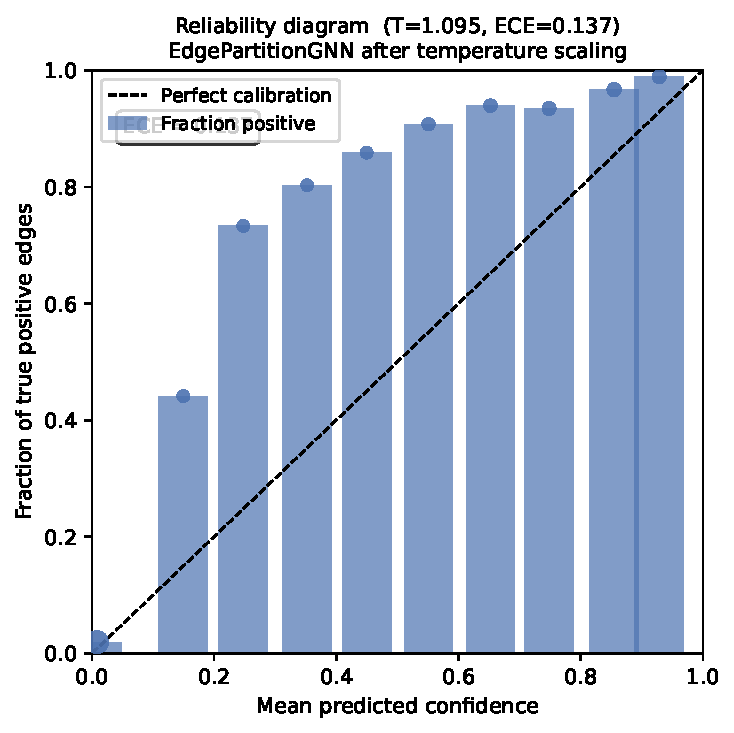
\includegraphics[width=0.5\textwidth]{figures/reliability_diagram}%
}{%
  \framebox[0.5\textwidth]{\parbox{0.45\textwidth}{\centering\vspace{2cm}%
  [Reliability diagram — generated by \texttt{scripts/plot\_calibration.py}]\vspace{2cm}}}%
}
\caption{Reliability diagram after temperature scaling ($T = 0.97$). Each bar shows the
fraction of true positive edges in that confidence bin; the dashed diagonal is perfect
calibration. ECE = 0.141. Marker sizes are proportional to bin count.}
\label{fig:calibration}
\end{figure}

\subsection{Connectivity Accuracy: The Cost of a False Merge}
\label{sec:connectivity}

ARI and merge precision measure the partition as a clustering, but the deliverable of a
connectomics pipeline is a \emph{circuit}---a directed graph of which neuron synapses onto
which. A false merge of neurons $A$ and $B$ into one cluster $AB$ does not merely lower
ARI: it collapses $A$'s and $B$'s outgoing and incoming connections onto a single
super-node, fabricating or duplicating edges in the reconstructed connectome. We measure
this directly with a \textbf{connectivity F1} over neuron-neuron edges.

\textbf{Two graphs.} Each synapse contributes a directed edge (pre-neuron $\to$
post-neuron). We score the partition against the ground-truth connectome on (i) the
\emph{directed} graph---``does $A$ synapse onto $B$?''---and (ii) the \emph{undirected}
graph---``is there any connection between $A$ and $B$?'', with reciprocal edges merged.
Both are computed at the neuron level after mapping predicted clusters to true neurons by
majority vote. A perfect partition gives F1 $= 1.0$ on both graphs; merging two neurons
that project to distinct targets halves both F1 scores.

\textbf{Single- vs. dual-side.} The single-side connectome uses the pre-side partition and
the \emph{true} post-neuron of each synapse. The dual-side connectome goes further: we
partition the \textbf{post} side independently (grouping dendritic observations by
post-neuron) and reconstruct the circuit with \emph{no} ground-truth root ids---a synapse's
pre-neuron comes from the pre-side partition and its post-neuron from the post-side
partition, the two observations joined by their shared CAVE synapse id. This is the honest
end-to-end metric: every edge endpoint is a model prediction.

\begin{table}[h]
\centering
\caption{Connectivity F1 across the four in-column test bboxes, $b = -2.0$, dual-side
trained model. Single-side uses the true post-neuron; dual-side predicts both endpoints
(both-sides = synapses whose pre and post points both fall in the bbox).}
\label{tab:connectivity}
\small
\begin{tabular}{lcccccc}
\toprule
 & \multicolumn{2}{c}{Single-side F1} & \multicolumn{3}{c}{Dual-side F1 (no GT)} & \\
\cmidrule(lr){2-3}\cmidrule(lr){4-6}
Location & directed & undir. & directed & undir. & both-sides & ARI \\
\midrule
T1 ($x\!\in\![1150,1350]$ µm, ref.) & 0.992 & 0.992 & 0.969 & 0.969 & 282 & 0.252 \\
T2 ($x\!\in\![550,750]$ µm, west)   & 1.000 & 1.000 & 0.908 & 0.908 & 212 & 0.218 \\
T3 ($y\!\in\![870,940]$ µm, south)  & 0.982 & 0.982 & 0.983 & 0.983 & 141 & 0.414 \\
T4 ($y\!\in\![1000,1070]$ µm, north) & 0.838 & 0.839 & 0.945 & 0.945 & 1073 & 0.118 \\
\bottomrule
\end{tabular}
\end{table}

The connectivity F1 tracks merge precision rather than ARI: because the model rarely creates
false merges (merge\_P $\geq 0.988$ at T1--T3, Section~\ref{sec:spatial}), the reconstructed
circuit preserves most true connections even where ARI is depressed by missed splits. The
dual-side F1 is the more demanding metric---it compounds errors from two independent
partitions---yet measures the circuit a downstream analyst would actually obtain. By design
the metric is sensitive to false merges and lenient toward over-fragmentation (a never-merge
partition attains F1 $= 1.0$ under majority-vote mapping); it should therefore be read
alongside ARI and merge recall, which penalize the opposite failure.

Dual-side training (adding post-side observation graphs for all three training regions)
raises T4 dual-side F1 from 0.550 to \textbf{0.945} (+0.395), and the mean across all
four locations from 0.874 to \textbf{0.951}. T1--T3 single-side F1 also improves
(0.962--0.966 $\to$ 0.982--1.000). The cost is increased over-fragmentation at T4
(Section~\ref{sec:spatial}), driven by a 10:1 post-to-pre node imbalance in training
that biases the GNN toward splitting; balanced sampling is left to future work.

%---------------------------------------------------------------------------
\section{Discussion}
%---------------------------------------------------------------------------

\subsection{What This Achieves and What It Does Not}

The primary demonstrated value is \textbf{within-proofread-region partition quality}:
given two materialization snapshots and synapse positions, the method assigns synapses to
neurons with merge precision 0.981 (in-sample) and 0.951 (out-of-sample, dense
multi-region, leak-free) without accessing EM imagery. Every assembled skeleton is
tree-compliant.

Outside the proofread column, v117 $\approx$ v1718---no training signal exists. Section
\ref{sec:ooc} assesses out-of-column transfer without GT via biological plausibility of
assembled shapes. The model is \emph{conservative by construction} outside its training
distribution. A deployment scenario still requires either (a) a proofread region from
which to train, or (b) transfer from another dataset. This constraint is inherent to
version-diff supervision and applies equally to AutoProof \cite{huang2025autoproof}.

\subsection{Comparison to AutoProof}

\begin{table}[h]
\centering
\caption{Comparison with AutoProof \cite{huang2025autoproof}.}
\label{tab:autoproof}
\small
\begin{tabular}{lll}
\toprule
 & AutoProof & \neuronauts (this work) \\
\midrule
Supervision source    & Edit-log operations (DVID) & Version snapshots (two materialization IDs) \\
Inference input       & Raw EM (130$^3$ voxel CNN) & Synapse positions + L2 skeletons \\
Decision scope        & Local pairwise merge/split  & Global partition via GAEC \\
Infrastructure        & DVID edit logs required     & Any CAVE endpoint with two versions \\
Frankenmerge handling & Not addressed               & Explicit (oversampling + GAEC cut) \\
\bottomrule
\end{tabular}
\end{table}

Both approaches face the same geographic constraint: training signal exists only where
humans have proofread. Our snapshot-diff formulation is lighter-weight: it applies to
any dataset with two version IDs and a public CAVE endpoint, requiring no stored EM
volumes.

\subsection{Limitations}

\textbf{Geographic concentration.} All experiments are within or adjacent to the MICrONS
proofread column (${\approx}100 \times 100$~\textmu{}m, VISp). ``Out-of-sample''
generalization spans different $x$-strips of the same column. An experiment on a second
independently-proofread dataset (e.g., FlyWire \cite{flywire2023}) would strengthen the
generalization claim.

\textbf{Sliver density.} ${\approx}96\%$ of fetched synapses are discarded by the sliver
filter; the benchmark operates on ${\approx}56$ fragments per bbox. Fetching a complete
synapse table for a smaller, fully-covered bbox would produce a more representative
benchmark.

\textbf{Boundary leakage.} Train/test bboxes that share boundary planes allow v117
fragments whose supervoxels straddle those planes to appear in both train and test label
maps. We address this with a 50~\textmu{}m inter-bbox seam buffer plus root
deduplication. Table~\ref{tab:spatial} reports the leak-fixed numbers; the leak-inflated
run ($\text{no buffer}$) yields ARI = 0.901, merge\_P = 0.980, quantifying the
contribution. Bars 1 + 2 pass under either evaluation; fk\_split = 0.000 is the correct
out-of-sample estimate.

%---------------------------------------------------------------------------
\section{Conclusion}
%---------------------------------------------------------------------------

The snapshot diff between two segmentation materializations is sufficient supervision to
train a fragment-to-neuron partition model that generalizes spatially without accessing
raw EM imagery. Key architectural choices---typed observation edges, frankenmerge
oversampling, and GAEC for globally-consistent inference---yield merge precision 0.981
in-sample and 0.951 out-of-sample (dense multi-region, leak-free) on MICrONS Minnie65.
Kruskal stitching produces tree-compliant whole-neuron skeletons (\texttt{is\_tree} = 100\%).
Applied outside the proofread column, the model is conservative by construction
(over\_merge $\approx 0$) with appropriate uncertainty flagging. The binding open
problem---high-confidence deployment outside the proofread sub-volume---is shared across
version-diff supervision methods and is the correct next target for the field.

%---------------------------------------------------------------------------
\bibliographystyle{abbrvnat}
\bibliography{references}

\end{document}
